\documentclass[table,dvipsnames]{beamer}
\mode<presentation>{
	\usetheme{Madrid}
	\setbeamercolor{title}{fg=Black,bg=Blue!15}
	\setbeamercolor{frametitle}{fg=Black,bg=Blue!15}
	\setbeamercolor{block title}{fg=Black,bg=Blue!15}
	\setbeamercolor{block}{fg=Black,bg=Blue!10}
}

\usepackage{graphicx}
\usepackage{booktabs}
\usepackage{xcolor}
\usepackage{multirow}
\usepackage{minted}
\usepackage[
type={CC},
modifier={by-sa},
version={4.0},
]{doclicense}

\definecolor{LightGray}{gray}{0.9}

\title[Rangkuman Kegiatan]{Rangkuman Diskusi Usulan Pengujian Prototype ke PT. Global Quality Indonesia}
\author{}
\institute[VibrasticLab : \ccbysa]{
	Achmadi ST MT\\
	\medskip
	\textit{}
}
\date{}

\begin{document}

	\begin{frame}
		\titlepage
	\end{frame}

	\begin{frame}
		\frametitle{Pihak Yang Terlibat}

		\begin{exampleblock}{Perwakilan Tim Audiometri}
			Mas Achmadi, ST MT selaku prototype engineer dari Tim Audiometri
		\end{exampleblock}

		\begin{exampleblock}{Perwakilan PT Global Quality Indonesia}
			Bapak Eliyana Firmansyah, ST MT selaku Contact Person dari PT Global Quality Indonesia
		\end{exampleblock}

		\begin{exampleblock}{Tentang PT Global Quality Indonesia}
			PT. GLOBAL QUALITY INDONESIA is a limited partnership which its main businesses include provision of Calibration, Material Testing, Training, Quality Management Consultant and Maintenance services.
		\end{exampleblock}

		\begin{exampleblock}{Website PT Global Quality Indonesia}
			\url{https://www.globalquality.co.id/}
		\end{exampleblock}
	\end{frame}

	\begin{frame}
		\frametitle{Pertemuan Pertama}

		\begin{exampleblock}{Uraian Ringkas}
			Pertemuan offline pertama telah dilaksanakan di kantor PT Global Quality Indonesia yang beralamat KOPO MAS REGENSI BLOK N - No. 7 C Bandung-Indonesia,
			dengan menunjukkan prototype produk yang akan dilakukan pengujian.
		\end{exampleblock}

		\begin{exampleblock}{Dokumentasi}
			\begin{center}
				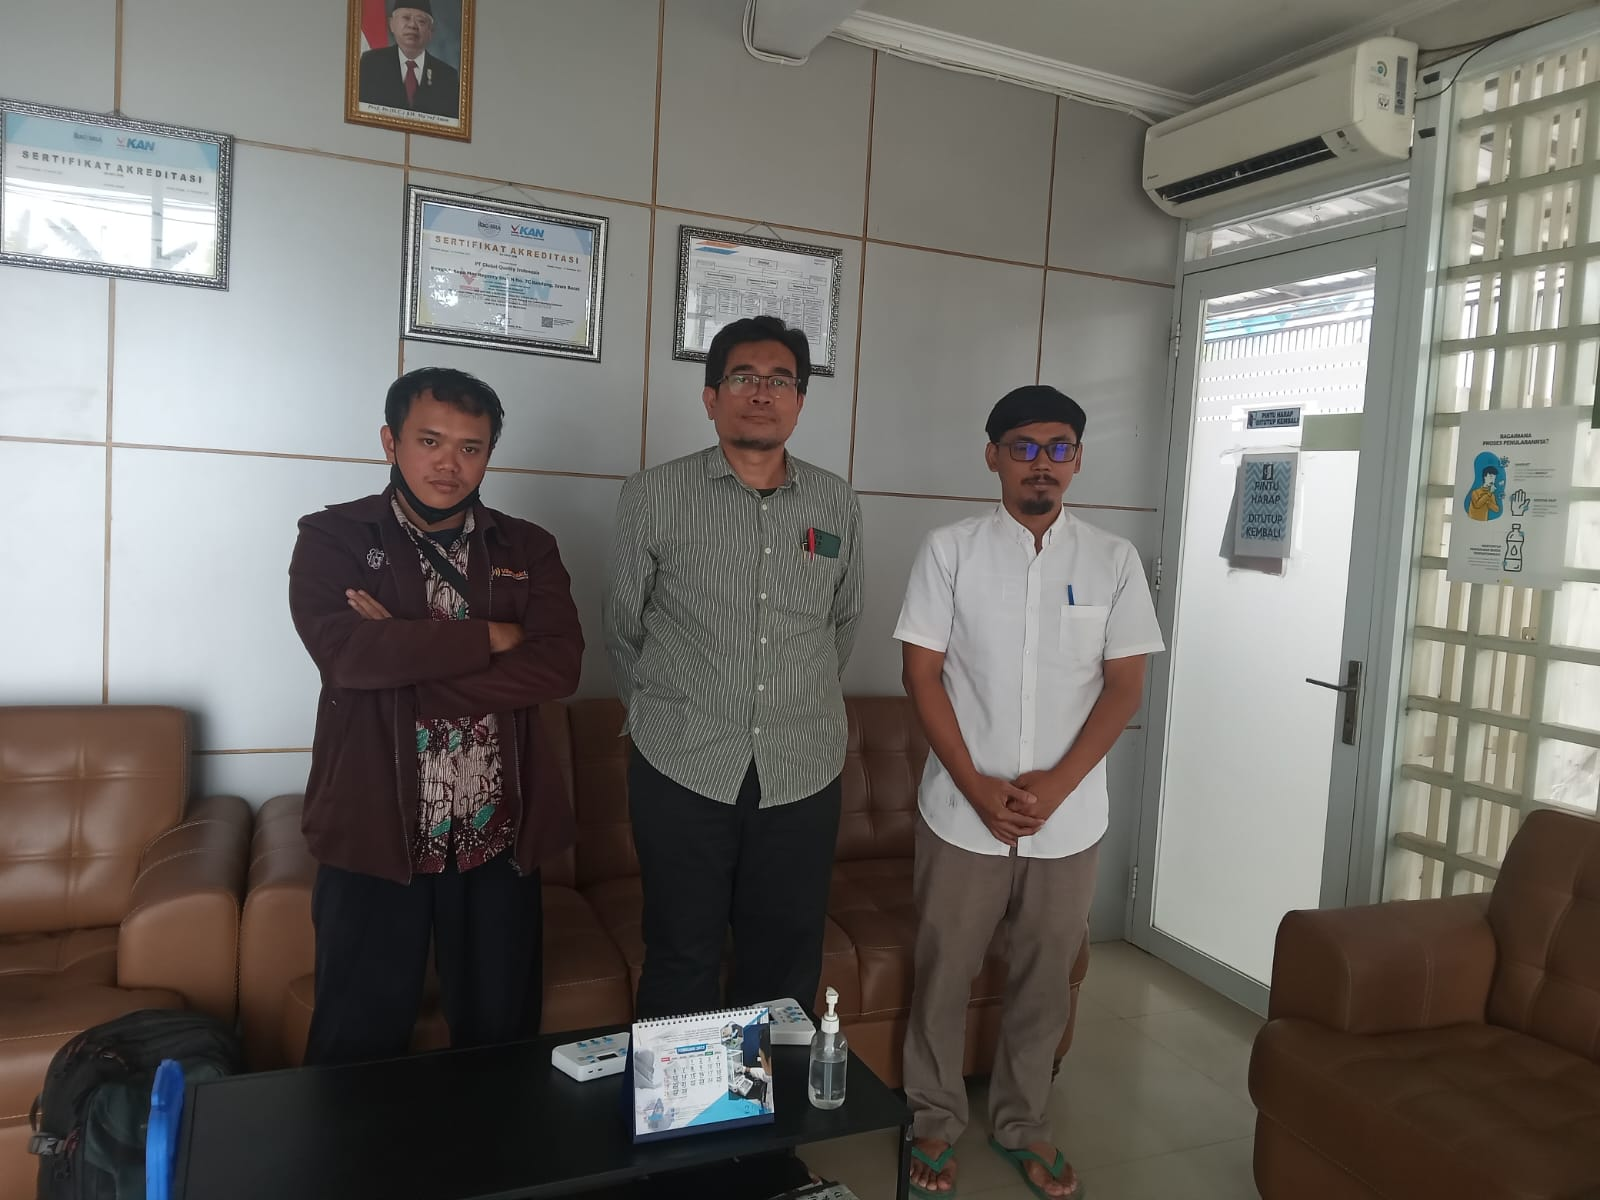
\includegraphics[width=150pt]{images/doc0}
			\end{center}
		\end{exampleblock}
	\end{frame}

	\begin{frame}
		\frametitle{Usulan Pengujian Metode Pengujian}

		\begin{exampleblock}{Uraian Ringkas}
			Pada tanggal 13 Maret 2023, diusulkan metode pengujian prototype menggunakan perangkat EARS (alih-alih menggunakan Sound Level Meter).
			Dicantumkan dokumen usulan berisi paparan bagaimana mengukur hasil nada murni menggunakan perangkat EARS.
		\end{exampleblock}

		\begin{exampleblock}{Dokumentasi}
			\begin{center}
				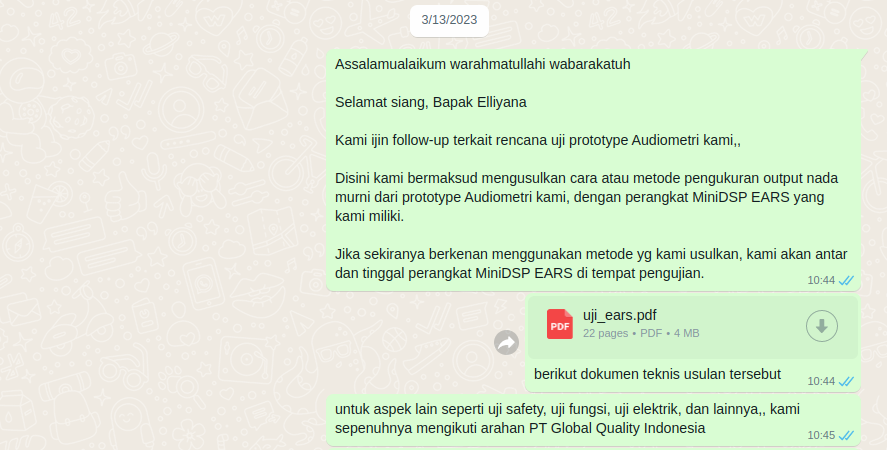
\includegraphics[width=200pt]{images/doc1}
			\end{center}
		\end{exampleblock}
	\end{frame}

	\begin{frame}
		\frametitle{Usulan Pengujian Metode Pengujian}

		\begin{exampleblock}{Uraian Ringkas}
			Sebagai respon, disampaikan oleh PT Global Quality Indonesia bahwa laboratorium yang tersedia tidak memiliki standarisasi dan pembanding dari perangkat EARS.
		\end{exampleblock}

		\begin{exampleblock}{Dokumentasi}
			\begin{center}
				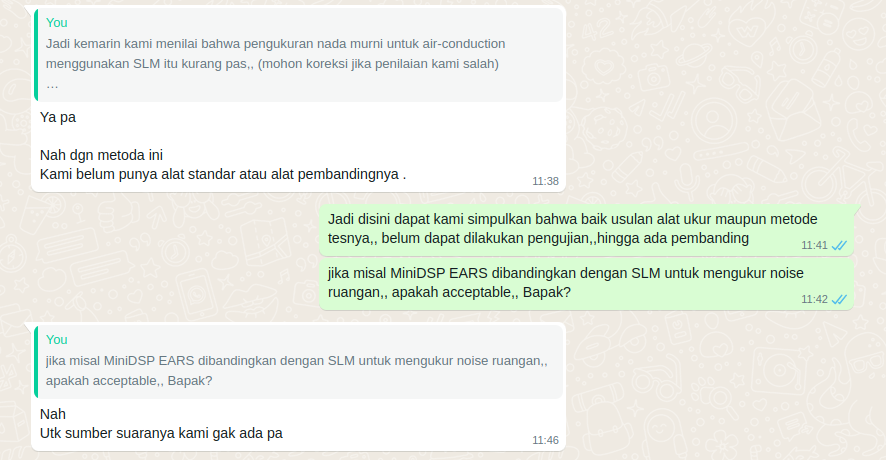
\includegraphics[width=200pt]{images/doc2}
			\end{center}
		\end{exampleblock}
	\end{frame}

	\begin{frame}
		\frametitle{Usulan Sound Level Meter sebagai Pembanding}

		\begin{exampleblock}{Uraian Ringkas}
			Sebagai kelanjutan, pada tanggal 15 Maret 2023 diusulkan metode perbandingan antara Sound Level Meter dan perangkat EARS.
			Dicantumkan dokumen usulan berisi paparan bagaimana membandingkan SLM dan EARS.
		\end{exampleblock}

		\begin{exampleblock}{Dokumentasi}
			\begin{center}
				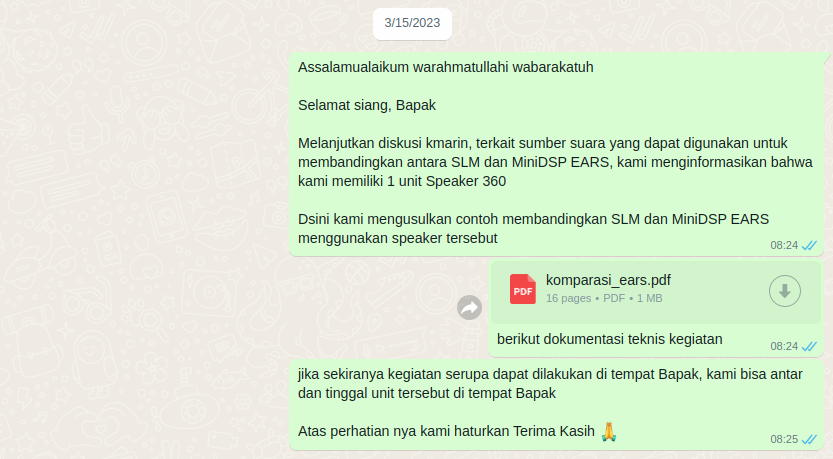
\includegraphics[width=200pt]{images/doc3}
			\end{center}
		\end{exampleblock}
	\end{frame}

	\begin{frame}
		\frametitle{Usulan Sound Level Meter sebagai Pembanding}

		\begin{exampleblock}{Uraian Ringkas}
			Sebagai respon, disampaikan oleh PT Global Quality Indonesia bahwa tidak ada standarisasi yang cocok digunakan untuk
			pengukuran Audiometri yang dapat dilakukan menggunakan perangkat EARS.
		\end{exampleblock}

		\begin{exampleblock}{Dokumentasi}
			\begin{center}
				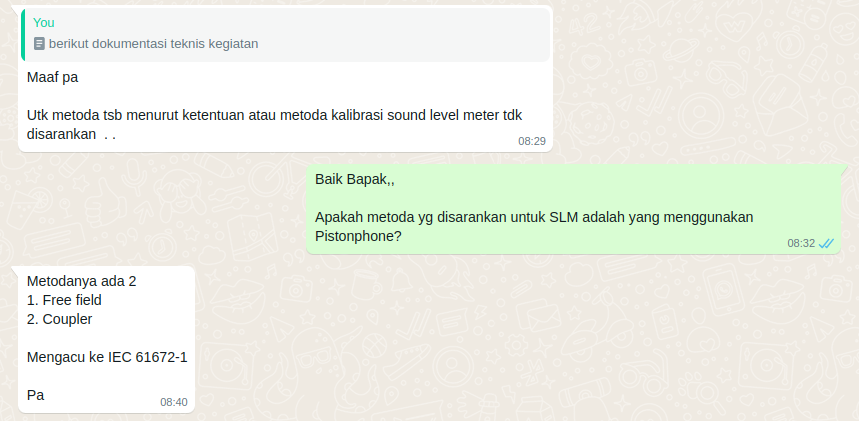
\includegraphics[width=200pt]{images/doc4}
			\end{center}
		\end{exampleblock}
	\end{frame}

	\begin{frame}
		\frametitle{Usulan Pengujian Mengikuti Laboratorium}

		\begin{exampleblock}{Uraian Ringkas}
			Tanggal 24 Maret 2023, diusulkan untuk pengujian prototype Audiometri dengan metode sepenuhnya mengikuti apa yang tersedia
			di Laboratorium PT Global Quality Indonesia.
		\end{exampleblock}

		\begin{exampleblock}{Dokumentasi}
			\begin{center}
				
\includegraphics[width=200pt]{images/doc5}
			\end{center}
		\end{exampleblock}
	\end{frame}

	\begin{frame}
		\frametitle{Usulan Pengujian Mengikuti Laboratorium}

		\begin{exampleblock}{Uraian Ringkas}
			Tanggal 28 Maret 2023, disepakati tidak ada kegiatan pengujian prototype Audiometri yang dapat dilakukan di PT Global Quality Indonesia.
		\end{exampleblock}

		\begin{exampleblock}{Dokumentasi}
			\begin{center}
				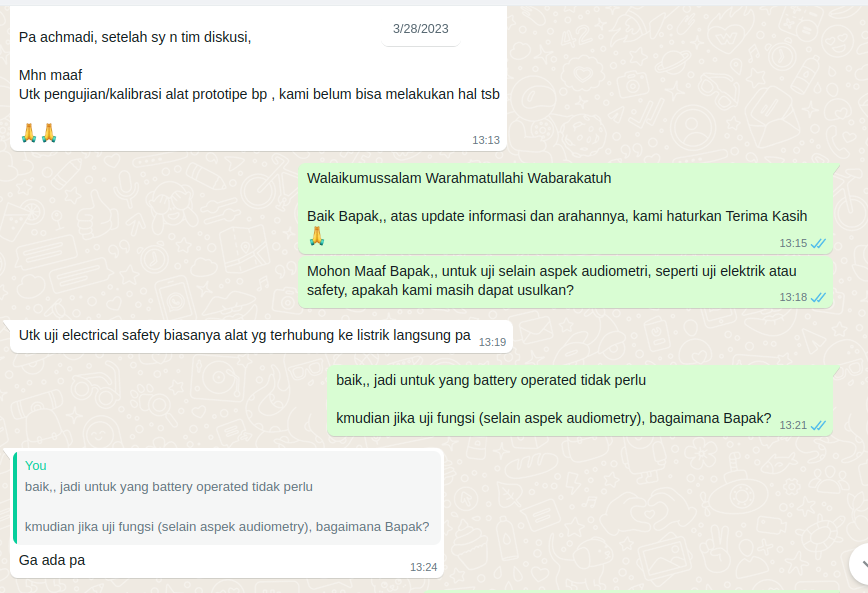
\includegraphics[width=200pt]{images/doc6}
			\end{center}
		\end{exampleblock}
	\end{frame}

\end{document}